\section{Annex}

\subsection{Figures}
\begin{table}[h]
\centering
\caption{DWG / DXF evaluation matrix.}
\label{tbl:DWGEvaluationMatrix}
\begin{tabular}{@{}llllllll@{}}
\toprule
Name         & Vendor         & Price        & Last Update      & License           & Read & Write & Comment                             \\ \midrule
YCAD Library & Ed Karlo       & -            & August 07, 2015  & LGPLv2            & Yes  & ?     & Very confusing \& no documentation. \\
Teigha       & ODA            & 2000 USD / Y &                  & Commercial        & Yes  & Yes   &                                     \\
Kabeja       &                & -            & March 12, 2008   & Apache License v2 & Yes  & No    &                                     \\
Tika         & Apache         & -            & October 19, 2016 & Apache License v2 & Yes* & No    & *Meta text reader.                  \\
jnetcad      & Johannes Raida & ?            & April 28, 2016   & Commercial        & Yes* & Yes*  & *Only converter for 3D Objects.     \\
CaffViewer   & DeCaff         & 1350 Euro    & May 17, 2016     & Freeware          & Yes  & Yes   &                                     \\ \bottomrule
\end{tabular}
\end{table}

\pagebreak
\subsection{Developer Guide}
This section describes, how to extend the application developed in this work. It is split into different tasks, which will most likely be done in the future.

\subsubsection{Adding new algorithm}
To add a new algorithm you have to create a new class, which implements the $IAlgorithm$ interface. The interface and algorithms are described in section~\ref{sub:algorithm}, but we will give you here a short overview over the interface and how to implement it.

We recommend, to split up different parts of a new process into different algorithms, which enhances the maintainability of an algorithm.

\begin{figure}[h]
  \centering
      \includegraphics[width=0.6\textwidth]{IAlgorithm_CD}
  \caption{Algorithm interface class diagram.}
  \label{fig:IAlgorithm_CD_DG}
\end{figure}

In figure~\ref{fig:IAlgorithm_CD_DG} you see the methods, which have to be implemented to run the algorithm. The very basic version of an algorithm just returns the input image as it is (Listing \ref{lst:basicAlgorithm}).

\begin{lstlisting}[caption={Basic version of an algorithm.}, label={lst:basicAlgorithm}, language=Kotlin]
class MyAlgorithm : IAlgorithm
{
    override val name: String
        get() = "MyAlgorithm"

    override fun run(image: AFImage, history: MutableList<AFImage>): AFImage {
        return image
    }
}
\end{lstlisting}

If you change the original image, it makes sense to create a copy of the incoming image, because the algorithm will maybe run multiple times. There are multiple ways to copy a $Mat$, but we have provided an extension method called $copy()$ (Listing~\ref{lst:extendedAlgorithm}, Line~\ref{line:AlgorithmCopy}), which creates a deep copy of the image.

If your algorithm uses parameters, which should be possible to change by the user, you can flag the parameter variables with an $AlgorithmParameter$ attribute (Listing~\ref{lst:extendedAlgorithm}, Line~\ref{line:AlgorithmParameter}). You then also have the possibility to set the range of the parameter and provide a short help text (Listing~\ref{lst:extendedAlgorithm}, Line~\ref{line:AlgorithmHelpText}). These informations will be read by the parameter window and shown during the process.

\begin{lstlisting}[caption={Extended version of an algorithm.}, label={lst:extendedAlgorithm}, language=Kotlin, escapechar=$]
class MyAlgorithm : IAlgorithm
{
    @AlgorithmParameter(name = "Threshold",
            minValue = 0.0,
            maxValue = 255.0,
            majorTick = 1.0,
            helpText = "Set the threshold value!") $\label{line:AlgorithmHelpText}$
    var threshold = 128.0 $\label{line:AlgorithmParameter}$

    override val name: String
        get() = "MyAlgorithm"

    override fun run(image: AFImage, history: MutableList<AFImage>): AFImage {
        val img = image.image.copy() $\label{line:AlgorithmCopy}$
        
        // do image processing
        img.threshold(threshold)

        history.add(AFImage(image.image, "Image before threshold")) $\label{line:AlgorithmHistory}$
        return AFImage(img, "Result")
    }
}
\end{lstlisting}

To provide images to the user from between the algorithm, you just have to add the image to the $history$ list (Listing~\ref{lst:extendedAlgorithm}, Line~\ref{line:AlgorithmHistory}). The images provided in there are shown in the parameter window (Section~\ref{sub:parameter_window}).

\subsubsection{Extending the user interface}

\begin{figure}[h]
	\centering
	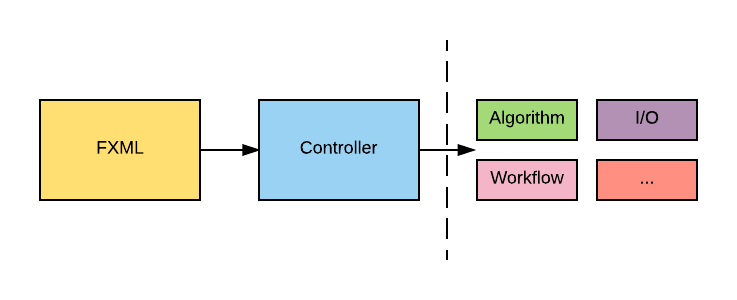
\includegraphics[width=0.8\textwidth]{fxmlArchitecture}
	\caption{User interface architecture.}
	\label{fig:fxmlArchitecture}
\end{figure}

\subsubsection{Training new classifiers}